\subsection*{Šmoulí super disko šou} % (fold)
\label{sub:šmoulí_super_disko_šou}

% subsection šmoulí_super_disko_šou (end)

Ke čtení článku doporučuji pustit hudební album, jehož název je shodný s názvem článku.
K nalezení je například zde: \url{https://cutt.ly/Pe5IGVZ}.

“Šmoulinka dnes vaří makarony, ví kdy je cedit, jak je voda osolená.”\\
“Vana příde v hod, když je špína z bot, padá a sám, všude na těle máš pot.”\\
“Jája je v koutku žumpy.”\\
“Ráda mám, když je brannej den já jsem vedoucí, ráda mám, když je brannej den tak tu velím jenom já!”

\begin{center}

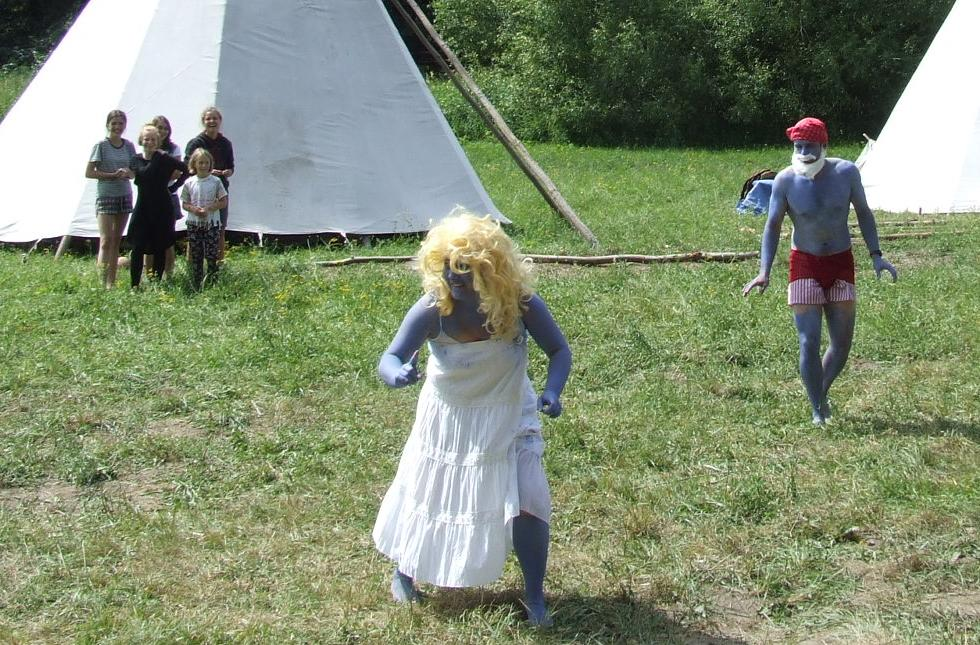
\includegraphics[width=7.5cm]{img/udo_clanky/smoulove.jpg}

\end{center}


Říkají vám něco tyto geniální texty? A taky jste si vždycky říkali, že by bylo super nechat děti běhat po louce a do toho jim pouštět hity z devadesátek přezpívané hlasy modrých tvorečků? No, jestli vás ne, mě jo.

Prostě se mi chtělo se natřít na modro, vzít si blonďatou paruku a chvíli si hrát na to, že jsem Šmoulinka. A to se mi splnilo, na táboře jsme si udělali branné dopoledne a velela jsem jenom já!

Přípravy programu vypadaly asi tak, že jsem všem uďům řekla, že udělám program, který bude modrý a dobrý, stáhla jsem si album, zařídila jsem papírové koule a koupila modrou barvu na tělo.

Tak jsme se s Vykačem a Humrem potkali v Hanyetu sněmáku a potřeli svá těla modří. Modří - Šmoulinka, Taťka Šmoula a DJ Šmoula jsme za zvuku šmoulí Mission Impossilbe epicky vyšli ze sněmáku a spustili šmoulí výcvik (teď už za zvuku Branného dne). Pak jsme děti rozdělili na čtvrtiny a vysvětlili jim, že je potřeba, aby běhali a přenášeli koule (šmouly) z různých území, a že je hodně důležité, aby u nich bylo nakonec šmoulů nejvíc. Přenášet mohli i Taťku (Humra) a ten byl za šmoulů deset.

A aby to běhání po louce nebylo jen tak nějaké běhání, jezdil mezi dětmi DJ Šmoula se svojí zvukomalebnou mašinou a pouštěl nám všechny ty báječné hity.

Sečteno a podtrženo, na tomto táboře se splnilo přání, které jsem už fakt dlouho měla a bylo to boží!


\podpis{Špunt}

\clearpage